% !TeX root = ../presentation.tex

\section{Introduction}
\begin{frame}{Interpolation overview}
	\begin{columns}[T] % align columns
		\begin{column}{.52\textwidth}
			\begin{itemize}
				\item Calculation of missing points using neighboring known points
				\item Vector to raster
				\item Raster to raster (Resampling)
				\item Spatial and spatio-temporal distributions of physical but also socioeconomic phenomena
				\item Deterministic vs Statistical
			\end{itemize}
		\end{column}%
		\hfill%
		\begin{column}{.48\textwidth}
			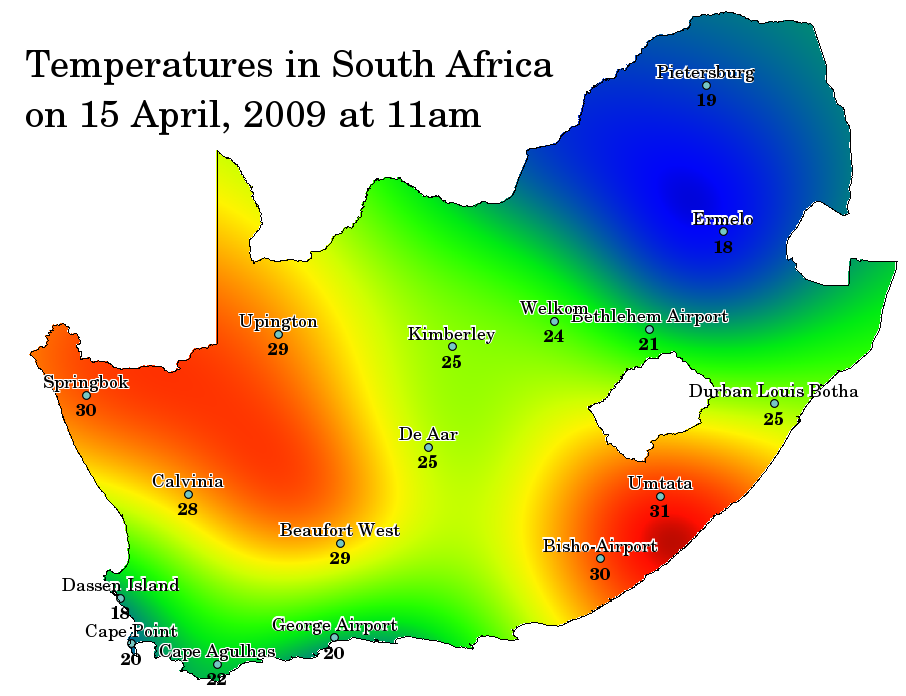
\includegraphics[width=\linewidth]{../writeup/images/temperature_map.png}\\
			\textit{\footnotesize Source: QGis Documentation\\11. Spatial Analysis (Interpolation)}
		\end{column}%
	\end{columns}
\end{frame}
\begin{frame}{The intra-urban heat islands effect}
	\begin{columns}[T] % align columns
		\begin{column}{.52\textwidth}
			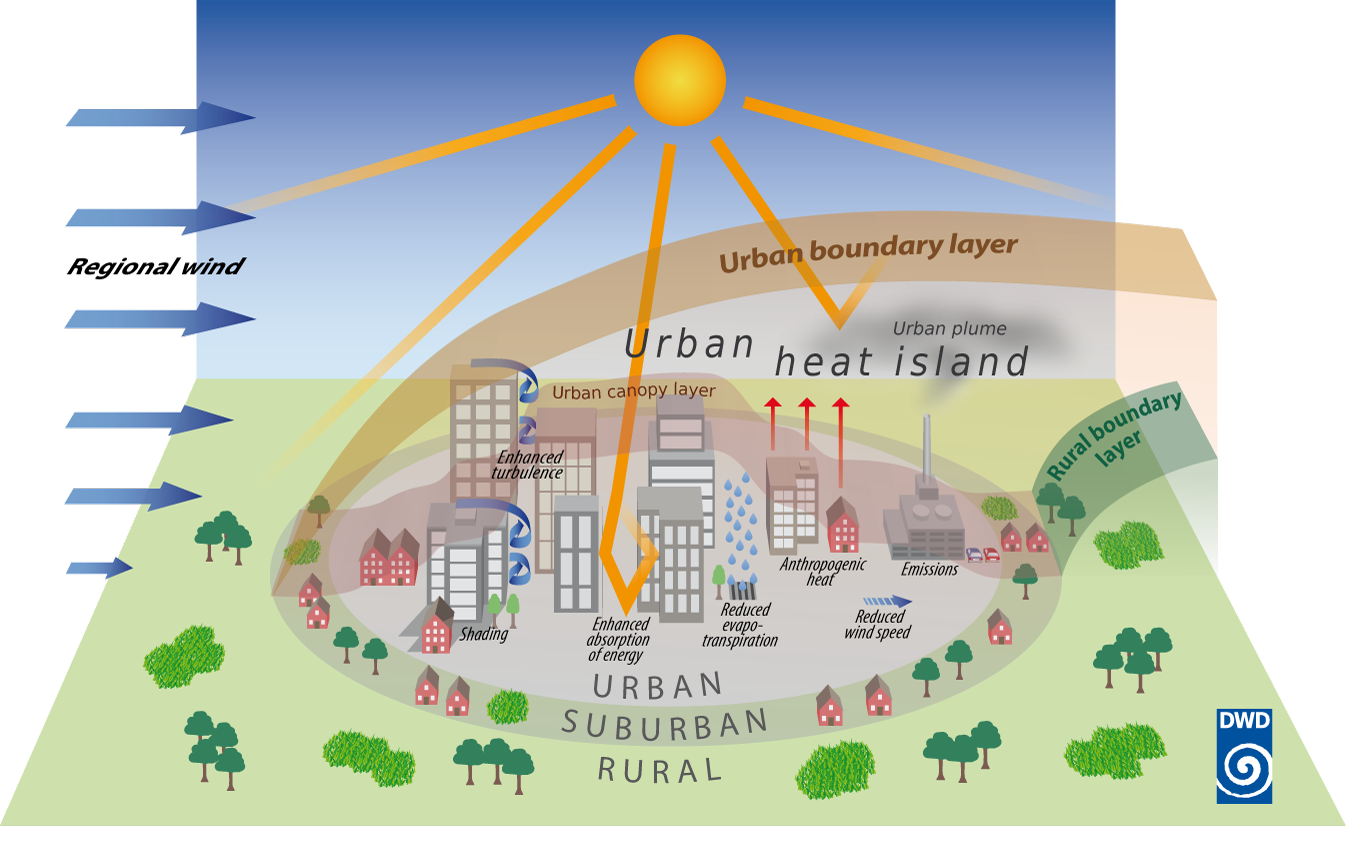
\includegraphics[width=\linewidth]{../writeup/images/urbanheatisland_01.png}\\
			\textit{\footnotesize Source: Deutscher Wetterdienst\\Urban climate - urban heat islands}
		\end{column}%
		\hfill%
		\begin{column}{.48\textwidth}
			\begin{itemize}
				\item \glqq{}{[\textellipsis]} an urban area or metropolitan area is significantly warmer than its surrounding rural areas due to human activities\grqq{}\cite{takebayashi_chapter_2020}
				# TODO: Statt UHI: Temperature differences within urban areas -> Intra-Urban Heat Islands (Bruns&Simko,2017)
				\item Infrastructure, such as buildings, roads and other sealed surfaces absorb and re-emit the sun's radiation in the form of heat
				\item natural landscapes, such as forests and water bodies have a cooling effect\cite{us_epa_learn_2014}
			\end{itemize}
		\end{column}%
	\end{columns}
\end{frame}
\begin{frame}{Project goals}
\begin{columns}[T] % align columns
	\begin{column}{.56\textwidth}
		\begin{itemize}
			\item Analyze temperature data from a citizen science project (openSenseMap)
			\item Visual product of the intra-urban heat islands effect
			\item Development over the course of the day
			\item Animation
		\end{itemize}
	\end{column}%
	\hfill%
	\begin{column}{.44\textwidth}
		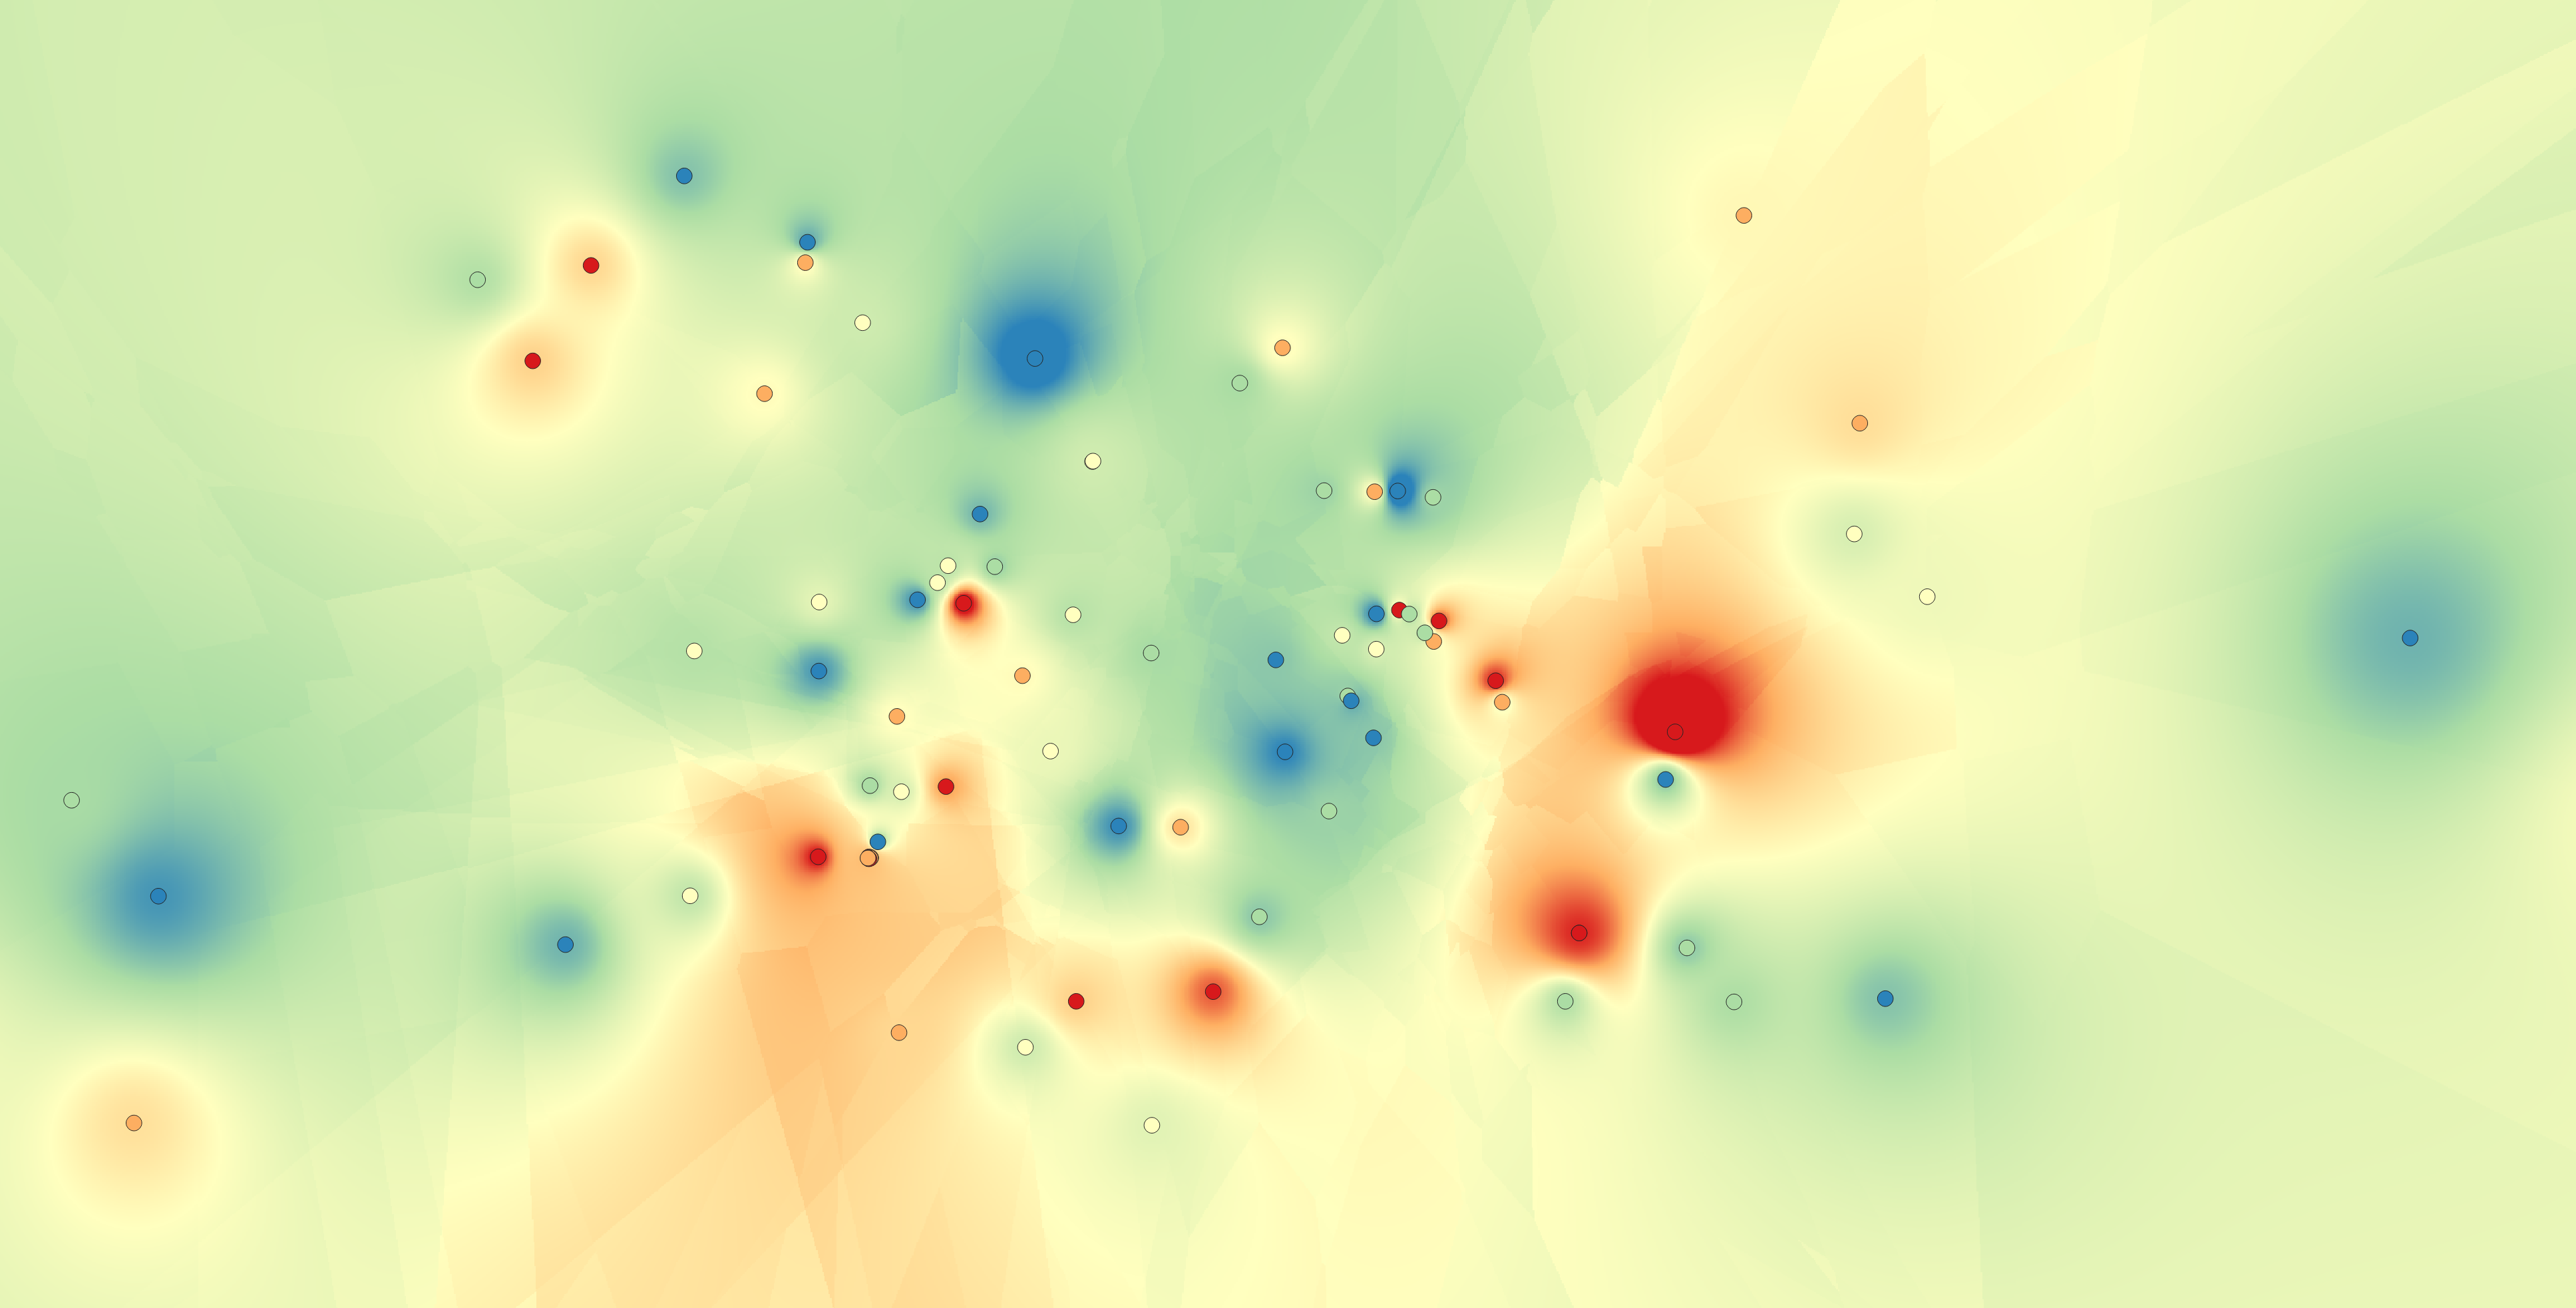
\includegraphics[width=\linewidth]{../writeup/images/interpolation_idw.png}\\
		\textit{\footnotesize Interpolation of temperatures between measurement stations}
	\end{column}%
\end{columns}
\end{frame}
